% !TeX spellcheck = en_US

\documentclass{../UTNetLab}

\title{The Web, DHCP, NTP and NAT}
\labnumber{8}
\newcommand\reference{
   S. Panwar, S. Mao, J.-dong Ryoo, and Y. Li, “The Web, DHCP, NTP and NAT,” in TCP/IP Essentials: A Lab-Based Approach, Cambridge: Cambridge University Press, 2004, pp. 159–186.
}

\begin{document}
\section*{Objectives}
\begin{itemize}
    \item The HyperText Transfer Protocol (HTTP) and the Apache web server.
    \item The Common Gateway Interface (CGI) and other web-server app (like PHP, Ruby, Python, \dots).
    \item The Dynamic Host Configuration Protocol (DHCP).
    \item The Network Time Protocol (NTP).
    \item The Network Address Translator (NAT) and the Port Address Translator (PAT).
    \item [-] An introduction to socket programming.
\end{itemize}
\part{HTTP Exercises}
For the exercises in this section, the network topology is simple with two hosts are connected to a single network segment with IP addresses, i.e.\  from 128.238.66.100 to 128.238.66.101.
You can use {Figure~3.server.gui}.

\begin{figure}[H]
    \centering
    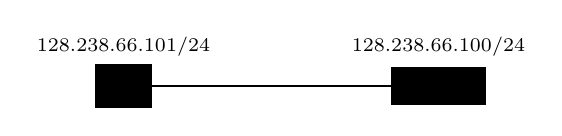
\begin{tikzpicture}
        \node[draw,fill=\colorhost] (Server) at (2,0){Server};
        \node[draw,fill=\colorhostgui] (gui) at (-2,0){gui};

        \draw (gui) -- (Server);
        \draw (Server) +(0,0.5) node {\scriptsize 128.238.66.100/24};
        \draw (gui) +(0,0.5) node {\scriptsize 128.238.66.101/24};

    \end{tikzpicture}
    \caption{One gui and one terminal host (Server) connected directly. (Figure~3.server.gui)}
    \label{fig:two-gui}
\end{figure}

\section{HTTP Server}
Examine the various configuration directives used and the corresponding settings\footnote{\path{/etc/apache2/apache2.conf}}.

Start the Apache server on the client host by: \lstbash{service apache2 start}.

\boxbash{{Server}'s Console}
\begin{lstlisting}
service apache2 start
\end{lstlisting}

In order to check if the server is working properly, you may start a \textit{Mozilla} web browser to download the test page at \lstgui{http://server.netlab/}.

\textbf{Note: } You should open \textit{gui}'s Console. This will open a VNC page in web browser of your operating system (by default, Mozilla Firefox). Then, from the start menu of the GUI, open \textit{Mozilla Firefox} and enter the \textit{Server}'s IP address in the URL box:

\boxgui{\textit{gui}'s web browser}
\begin{lstlisting}
http://128.238.66.100/
\end{lstlisting}

Then, execute the following command in \textit{Server} to list the process IDs of the \lstbash{apache2} processes started:

\boxbash{{{Server}'s Console}}
\begin{lstlisting}
pgrep apache2
\end{lstlisting}

Open the Multi-Processing Module config file with a text editor and study its various configurations and their applications by executing:

\boxbash{{Server}'s Console}
\begin{lstlisting}
nano /etc/apache2/mods-available/mpm_prefork.conf
\end{lstlisting}

\textbf{Note: } To search for a string in \lstbash{nano}, use \lstbash{Ctrl+W}

Save the output and the configuration file for the lab report.

\begin{report}
    \item How many \lstbash{apache2} processes were started?
    Which one was the master server, and which ones were the child servers?
    Use \lstbash{htop} in the \textbf{tree} mode to see process hierarchy by executing:
    
\boxbash{{Server}'s Console}
\begin{lstlisting}
htop --tree
\end{lstlisting}

    Justify your answer using the \textbf{apache2} configurations file.
    Explain your answer with value of \textit{StartServers, MinSpareServers, MaxSpareServers, MaxRequestWorkers, ServerLimit, MaxConnectionsPerChild}\footnote{Need to read \textit{Apache} web documents}.

    \item What is the purpose of initiating multiple apache2 processes?
\end{report}

\section{HTTP Request}
Execute \lstbash{wireshark} to capture packets between the \textit{gui} host and the \textit{server} host.

Connect to the \textit{server} host’s web server from the \textit{gui}'s terminal:

\boxbash{{gui's Auxiliary Console}}
\begin{lstlisting}[emph={server,netlab}]
telnet server.netlab 80
\end{lstlisting}

In the telnet console, type the following HTTP request line by line:

\boxbashaux{{gui's Auxiliary Console -> \textbf{telnet}}}
\begin{lstlisting}[language={HTTP},morekeywords={[2]GET,From,User-Agent},escapechar=*,emph={server,netlab},breaklines=true,breakatwhitespace=true,]
GET /index.html HTTP/1.0
From: netlab@server.netlab
User-Agent: HTTPTool/1.0
*\newline*
*\newline*
\end{lstlisting}

Note that you need to press the \textit{Return} (\textit{Enter}) key to input the last line, which is blank (you should press the \textit{Enter} key twice).
When the \lstbash{telnet} process is terminated, save the output for your lab report.

Terminate \lstbash{wireshark} and analyze the captured HTTP packets.
Print and save the HTTP request and response.

Save the HTTP response’s data part into a file, named \path{index.html}.
Use \textit{Mozilla} to view the file.

\begin{report}
    \item Submit the HTTP request and response, including the start-lines and all the headers.
\end{report}


\section{HTTP \texttt{Keep-Alive}}
By default, \textit{Apache} server supports persistent connections. Before this exercise, check the \texttt{KeepAlive} directive in the server configuration file\footnote{\path{/etc/apache2/apache2.conf}} to make sure it is turned on as \lstconf{KeepAlive On}.
To do this, execute the following command and use \lstbash{Ctrl+W} to search for \lstconf{KeepAlive}:

\boxbash{{Server}'s Console}
\begin{lstlisting}
nano /etc/apache2/apache2.conf
\end{lstlisting}

Execute \lstbash[emph={gui,server,netlab},morekeywords={[3],host,and}]{tcpdump host gui.netlab and server.netlab} or run \lstbash{wireshark} to capture packets between the \textit{gui} host and the \textit{server} host.

\boxbashaux{{Server}'s Auxiliary Console}
\begin{lstlisting}
tcpdump host 128.238.66.100 and 128.238.66.101  # or run wireshark
\end{lstlisting}

Open web console of the \textit{gui}'s host.
In the remove console, open \textit{Mozilla} \lstbash{firefox} application.


Enter the URL \lstgui{http://server.netlab/try1.html}in the \textit{gui} NoVNC's web browse, to download the HTML file consisting a line of text, an embedded picture, and a hyperlink.

\boxgui{gui's web browser}
\begin{lstlisting}
http://server.netlab/try1.html   # or http://128.238.66.100/try1.html
\end{lstlisting}

In \textit{Server}, disable the \textit{Apache} server persistent connections by changing the value of \texttt{KeepAlive} option to \lstbash{Off} from the configuration file (as mentioned above). To save the file after modifying it, press \lstbash{Ctrl+X}, confirm it by entering \lstbash{Y} and press enter. Then restart \lstbash{apache2} service by running following command:

\boxbash{{Server}}
\begin{lstlisting}
service apache2 restart
\end{lstlisting}

Use \lstbash{tcpdump} or run \lstbash{wireshark} and print the HTTP requests and responses for the lab report.

Use \textit{Mozilla} in the \textit{gui}'s to reload the \lstgui{try1.html} file.
Use \textit{Ctrl+F5} to ignore cache.

Use \lstbash{wireshark} and print the HTTP requests and responses for the lab report.

\begin{report}
    \item When you browsed the \path{try1.html} file for the first time, how many HTTP requests were sent?
    Which files were requested?
    How many TCP connections were used?

    \item Answer the above questions for when you browsed the \path{try1.html} file for the second time.

    \item What is the purpose of using persistent connections?
\end{report}

\section{HTTP Submit}
Execute \lstbash{wireshark} to capture packets between the \textit{gui} host and the \textit{server} host.

Use \textit{Mozilla} \lstbash{firefox} in the (\textit{gui}) to download the \lstgui{http://server.netlab/try2.htm} file  from the server, which is an \textit{HTML} form.

\boxgui{\textit{gui}'s web browser}
\begin{lstlisting}
http://128.238.66.100/try2.html
\end{lstlisting}

Fill the input line in the form, such as \textit{netlab} or \textit{hostname} and click the submit button.

When the server response is received, terminate \lstbash{wireshark}.

Examine how LAMP (for php)\footnote{or CGI (for perl)} works, and identify the data string sent to the server.
Save the HTTP request containing the data string for lab report.

\begin{report}
    \item Submit the data string sent to the server.
\end{report}

\part{DHCP Exercises}
For the exercises in this section, the network topology is given in \hyperref[fig:1.3]{Figure~1.3}, where all the hosts are connected to a single network segment.

\begin{center}
    \begin{minipage}{0.48\textwidth}
        \begin{flushright}
            \begin{figure}[H]
                \centering
                
\begin{tikzpicture}
                    \node[draw,align=center,rounded corners,fill=\colorswitch] (s) at (0,0){Core\\Switch};
                    \node[draw,fill=\colorhost] (h0) at (0,2){h0};
                    \node[draw,fill=\colorhost] (h1) at ({sqrt(2)},{sqrt(2)}){h1};
                    \node[draw,fill=\colorhost] (h2) at (2,0){h2};
                    \node[draw,fill=\colorhost] (h3) at (-{sqrt(2)},{sqrt(2)}){h3};
                    \node[draw,fill=\colorhost] (h4) at (-2,0){h4};
                    \node[draw,fill=\colorhost] (h5) at (-{sqrt(2)},-{sqrt(2)}){h5};
                    \node[draw,fill=\colorhost] (h6) at (0,-2){h6};
                    \node[draw,fill=\colorhost] (h7) at ({sqrt(2)},-{sqrt(2)}){h7};

                    \draw (h0) -- (s);
                    \draw (h1) -- (s);
                    \draw (h2) -- (s);
                    \draw (h3) -- (s);
                    \draw (h4) -- (s);
                    \draw (h5) -- (s);
                    \draw (h6) -- (s);
                    \draw (h7) -- (s);
                \end{tikzpicture}
                \caption{A single segment network (Figure~1.3)}
                \label{fig:1.3}
            \end{figure}
        \end{flushright}
    \end{minipage}
\end{center}

\section{DHCP Server}
In this exercise, we use \textit{h1} as the DHCP server, with a configuration file\footnote{\path{/etc/dhcp/dhcpd.conf}} shown in \hyperref[tab:8.3]{Table~8.3}.
Configure the DHCP server by opening the configuration file with a text editor such as \lstbash{nano}.
To do this, run the following command:

\boxbash{{h\textsubscript{1}}'s Console}
\begin{lstlisting}
echo > /etc/dhcp/dhcpd.conf # clear file
nano /etc/dhcp/dhcpd.conf   # edit file and save (Ctrl+X)
\end{lstlisting}

Do the following:

\begin{enumerate}
    \item Change MAC address of \textit{h5} in server configuration file (\hyperref[tab:8.3]{Table~8.3}) by your \textit{h5} MAC address and save to \textit{dhcpd.conf}.

          \textbf{Note: }to obtain MAC address of \textit{h5} run the following command:

          \boxbash{{h\textsubscript{5}}'s Console}
          \begin{lstlisting}
ifconfig
          \end{lstlisting}

    \item Set IP of \textit{h1} to {128.238.66.100}
 
          \boxbash{{h\textsubscript{1}}'s Console}
          \begin{lstlisting}
ifconfig eth0 128.238.66.100/24
   	      \end{lstlisting}


    \item Start the DHCP server on \textit{h1} in the foreground and working in the debugging mode:

          \boxbash{{h\textsubscript{1}}'s Console}
          \begin{lstlisting}
dhcpd -d -f
          \end{lstlisting}


    \item Execute \lstbash{tcpdump -exn -nn -s 100} or \lstbash{wireshark} to capture the DHCP messages in the network segment.

          \boxbashaux{{h\textsubscript{1}}'s Auxiliary Console}
          \begin{lstlisting}
tcpdump -exn -nn -s 100			# or run wireshark
          \end{lstlisting}

    \item Then do the following to enable DHCP for the Ethernet interface on the \textit{h2}.

          Run \lstbash{ifconfig eth0 0} on \lstbash{h2} to clear IP of \textit{eth0}.
          And run \lstbash{dhclient eth0}.

          \boxbash{{h\textsubscript{2}}'s Console}
          \begin{lstlisting}
ifconfig eth0 0
dhclient eth0
          \end{lstlisting}

          When \textit{h0} is successfully reconfigured, execute \lstbash{ifconfig -a} or \lstbash{ip a} to display its
          network interface configurations and execute \lstbash{netstat -rn} or \lstbash{ip r} to display its routing table.

          \boxbash{{h\textsubscript{2}}'s Console}
          \begin{lstlisting}
# see ip and subnet
ifconfig -a # or  ip a
# see routing
netstat -rn # or  ip r
          \end{lstlisting}

          Save the outputs for the lab report.

    \item Then, repeat 5 for the \textit{h3}.

    \item Repeat 5 for the \textit{h4}.

    \item Repeat 5 for the \textit{h5}.
\end{enumerate}

Terminate \lstbash{wireshark}.
Print out the DHCP messages for the lab report.

Save the DHCP server output on the \textit{h1} for the lab report.

\boxconf{/etc/dhcp/dhcpd.conf}
\begin{lstlisting}[language={conf}, caption={A DHCP server configuration file (Table~8.3)\label{tab:8.3}},emph={xx}]
default-lease-time 600;
max-lease-time 7200;
option subnet-mask 255.255.255.0;
option broadcast-address 128.238.66.255;
option routers 128.238.66.1;
#option domain-name-servers 128.238.2.38, 128.238.3.21;
#option domain-name "netlab.ut.ac.ir";

subnet 128.238.66.0 netmask 255.255.255.0 {
    range 128.238.66.111 128.238.66.112;
}

host h5 {
    hardware ethernet xx:xx:xx:xx:xx:xx;   #Change this with h5's MAC address
    fixed-address 128.238.66.110;
}
\end{lstlisting}

\begin{report}
    \item Compare the DHCP operation captured by \lstbash{wireshark} and that shown by the DHCP server output.
    Explain how DHCP works.

    \item Did \textit{h2} and the \textit{h3} successfully obtain a set of new parameters?
    Compare the \lstbash{ifconfig} and \lstbash{netstat} output with the parameters carried in the corresponding DHCP messages.

    \item Answer the above question for the \textit{h4}.
    Explain why \textit{h4} failed.

    \item Answer the above question for the \textit{h5}.
    Explain why \textit{h5} succeeded.
\end{report}

\part{NTP exercises}
Before proceeding to the next exercise, reboot the hosts and set network topology is given in \hyperref[fig:1.3]{Figure~1.3} and set hosts IP address from 128.238.66.100 to 128.238.66.107.
\begin{center}
    \begin{minipage}{0.48\textwidth}
        \begin{flushleft}
            \begin{table}[H]
                \caption{The IP addresses of the hosts (Table~1.2)}
                \centering
                \begin{tabular}{ c c c }
                    \hline \hline
                    Host & IP Address     & Subnet Mask   \\
                    \hline
                    h0   & 128.238.66.100 & 255.255.255.0 \\
                    h1   & 128.238.66.101 & 255.255.255.0 \\
                    h2   & 128.238.66.102 & 255.255.255.0 \\
                    h3   & 128.238.66.103 & 255.255.255.0 \\
                    h4   & 128.238.66.104 & 255.255.255.0 \\
                    h5   & 128.238.66.105 & 255.255.255.0 \\
                    h6   & 128.238.66.106 & 255.255.255.0 \\
                    h7   & 128.238.66.107 & 255.255.255.0 \\
                    \hline \hline
                \end{tabular}
            \end{table}
        \end{flushleft}
    \end{minipage}
\end{center}

\section{Local Date}
Execute \lstbash{date} to display the system time of your host.
Display the manual page of \lstbash{date}, and study its options and usages.
Try the following \lstbash{date} commands:

\boxbash{{h\textsubscript{0}}'s Console}
\begin{lstlisting}[emph={$file-name}]
date --date='2 days ago'
date --date='3 months 2 days'
date --set='+3 minutes'
date -r $file-name # for example: /etc/network/interfaces
    \end{lstlisting}
You can choose any file in the current directory for the \textit{file-name} parameter\footnote{Like \path{/etc/network/interfaces}.}.

\begin{report}
    \item Submit the \lstbash{date} outputs you saved.
    Explain the use of the commands.
\end{report}

\section{Remote Date}
While \lstbash[emph={h0,h1,netlab}]{tcpdump -n -nn -ex host h0.netlab and h1.netlab} or \lstbash{wireshark} is running, execute \lstbash[emph={h1,netlab}]{rdate -p h1.netlab} on the \textit{h0} to display the system time of the \textit{h1} machine.
Repeat the above \lstbash{rdate} command, but use the \lstbash{-u} option.

\boxbashaux{{h\textsubscript{0}}'s Auxiliary Console}
\begin{lstlisting}
tcpdump -n -nn -ex host 128.238.66.100 and 128.238.66.101		# or run wireshark
\end{lstlisting}

\boxbash{{h\textsubscript{0}}'s Console}
\begin{lstlisting}
rdate -p 128.238.66.101
\end{lstlisting}

Now, repeat the above \lstbash{rdate} command but use the \lstbash{-u} option:

\boxbash{{h\textsubscript{0}}'s Console}
\begin{lstlisting}
rdate -p 128.238.66.101 -u
\end{lstlisting}

Save the \lstbash{wireshark} or \lstbash{tcpdump} outputs for the lab report.

\begin{report}
    \item What port numbers were used by the \textit{h1} (server) machine?
    What port numbers were used by the \textit{h0} (client) host?

    \item How many bytes of data (application data) were returned by the \textit{h1} time server, both in the UDP case and in the TCP case?

    \item What TCP header options were used?
\end{report}

\section{NTP Sync}
In this exercise, we start the NTP server daemon on the \textit{h0} and use NTP to synchronize all the other hosts to \textit{h0}.
Study the NTP configuration file \path{/etc/ntp.conf} in the \textit{h0} and in your host.

\boxbash{{h\textsubscript{0}}'s Console}
\begin{lstlisting}
less /etc/ntp.conf # can use "nano" or "vim"
# press 'q' to exit
\end{lstlisting}

Start the NTP server on the \textit{h0} by \lstbash{service ntp start}.
To determine the status of the NTP server, use \lstbash{service ntp status}.

\boxbash{{h\textsubscript{0}}'s Console}
\begin{lstlisting}
service ntp start
service ntp status
\end{lstlisting}

Use \lstbash[emph={h0,h1,netlab},morekeywords={[3],host,and}]{tcpdump -ex -n -nn host h1.netlab and h0.netlab} or \lstbash{wireshark} to capture packets between the \textit{h1} host and the \textit{h0}.

\boxbashaux{{h\textsubscript{1}}'s Auxiliary Console}
\begin{lstlisting}
tcpdump -ex -n -nn host 128.238.66.101 and 128.238.66.100   # or run wireshark
\end{lstlisting}

Execute \lstbash{ntpdate -d -v 128.238.66.100} to synchronize the \textit{h1} host with \textit{h0}.

\boxbash{{h\textsubscript{1}}'s Console}
\begin{lstlisting}
ntpdate -d -v 128.238.66.100
\end{lstlisting}

Study the output of this command.
Save the \lstbash{ntpdate} and the \lstbash{wireshark} outputs for the lab report.

\begin{report}
    \item Which port does the NTP server use?
    Justify your answer using the \lstbash{wireshark} output.
\end{report}

\section{** NTP Server}
Keep the NTP server running on the \textit{h0}.
Execute \lstbash[emph={h1,h0,netlab},morekeywords={[3]host,and}]{tcpdump -exn -nn host h1.netlab and h0.netlab} or \lstbash{wireshark} to capture the NTP messages between the \textit{h1} host and the \textit{h0}.

\boxbashaux{{h\textsubscript{1}}'s auxiliary console}
\begin{lstlisting}
tcpdump -exn -nn host 128.238.66.101 and 128.238.66.100 # or run wireshark
\end{lstlisting}

Edit the \path{/etc/ntp.conf} in \textit{h1} and add \lstconf{server 128.238.66.100} to config file.

\boxbash{{h\textsubscript{1}}'s Console}
\begin{lstlisting}
echo "server 128.238.66.100" > /etc/ntp.conf
\end{lstlisting}

Start the NTP client on the \textit{h1}, by executing:

\boxbash{{h\textsubscript{1}}'s Console}
\begin{lstlisting}
service ntp start
\end{lstlisting}

Wait for several minutes.
Then terminate the \lstbash{tcpdump} program.
Analyze the captured NTP packets.
Print one of the NTP packets for the lab report.

Execute \lstbash{ntpq -p} on the \textit{h1} to get \lstbash{ntp} server list.

\boxbash{{h\textsubscript{1}}'s Console}
\begin{lstlisting}
ntpq -p
\end{lstlisting}

Execute \lstbash{ntptrace} on the \textit{h1} to show the client/server relation of NTP.

\boxbash{{h\textsubscript{1}}'s Console}
\begin{lstlisting}
ntptrace
\end{lstlisting}


\begin{report}
    \item Submit the NTP packet captured.
    List the fields and their values.

    \item What was the rate at which NTP queries were sent by the client?

    \item Which stratum was your host in? Which stratum was the NTP server in?
\end{report}

\part{NAT Exercises}
For the exercises in this section, we use a network setting as shown in \hyperref[fig:8.7]{Figure~8.7}.
The lower subnet is a private network where the hosts are assigned with the Class A addresses with the 10.0.0.0/8 prefix.
The upper subnet represents the Internet.
The hosts, i.e.\  \textit{h0} and the \textit{h1} are assigned with public IP addresses.
Router 1 is used as the stub router, which performs address or port translation for the private network.
\begin{figure}[H]
    \centering
    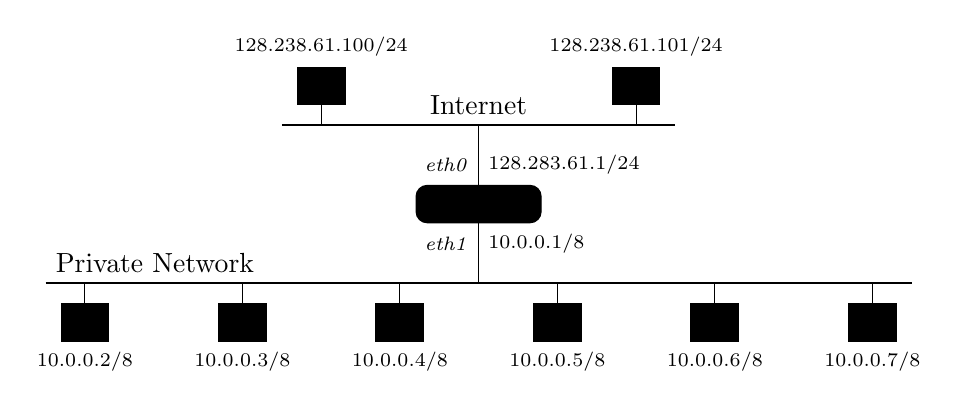
\begin{tikzpicture}
        \draw (0,0) node[draw,rounded corners,fill=\colorrouter] (r1) {Router 1}
        -- +(0,1)
        -- +(0,-1)
        +(0,0.5) node[anchor=east] {\scriptsize\textit{eth0}}
        +(0,0.5) node[anchor=west] {\scriptsize128.283.61.1/24}
        +(0,-0.5) node[anchor=east] {\scriptsize\textit{eth1}}
        +(0,-0.5) node[anchor=west] {\scriptsize10.0.0.1/8}
        ;
        \draw (-1*2,1.5) node[draw,fill=\colorhost] (h0) {h0}
        -- +(0,-0.5)
        +(0,0.5) node {\scriptsize 128.238.61.100/24}
        ;
        \draw (1*2,1.5) node[draw,fill=\colorhost] (h1) {h1}
        -- +(0,-0.5)
        +(0,0.5) node {\scriptsize 128.238.61.101/24}
        ;
        \draw (-3*2+1,-1.5) node[draw,fill=\colorhost] (h2) {h2}
        -- +(0,0.5)
        +(0,-0.5) node {\scriptsize 10.0.0.2/8}
        ;
        \draw (-2*2+1,-1.5) node[draw,fill=\colorhost] (h3) {h3}
        -- +(0,0.5)
        +(0,-0.5) node {\scriptsize 10.0.0.3/8}
        ;
        \draw (-1*2+1,-1.5) node[draw,fill=\colorhost] (h4) {h4}
        -- +(0,0.5)
        +(0,-0.5) node {\scriptsize 10.0.0.4/8}
        ;
        \draw (1*2-1,-1.5) node[draw,fill=\colorhost] (h5) {h5}
        -- +(0,0.5)
        +(0,-0.5) node {\scriptsize 10.0.0.5/8}
        ;
        \draw (2*2-1,-1.5) node[draw,fill=\colorhost] (h6) {h6}
        -- +(0,0.5)
        +(0,-0.5) node {\scriptsize 10.0.0.6/8}
        ;
        \draw (3*2-1,-1.5) node[draw,fill=\colorhost] (h7) {h7}
        -- +(0,0.5)
        +(0,-0.5) node {\scriptsize 10.0.0.7/8}
        ;
        \draw[thick] (-2-0.5,1) -- +(2*2+1,0) node[pos=0.5,above] {Internet};
        \draw[thick] (-6+0.5,-1) -- +(6*2-1,0) node[pos=0,above,anchor=south west] {Private Network};
    \end{tikzpicture}
    \caption{The network configuration for the NAT exercises (Figure~8.7)}
    \label{fig:8.7}
\end{figure}

\section{NAT}
Connect the hosts and Router 1 as shown in \hyperref[fig:8.7]{Figure~8.7}.
Then set the IP address and the network mask of your host as shown in the figure.
In addition, you need to add a default route in your host’s routing table, using the router interface on your subnet as the default router.
Open the router console and configure the router as shown in \hyperref[tab:8.5]{Table~8.5}.
Note that there is a static translation that maps 10.0.0.7, or the \textit{h7}, to 128.238.61.104.
Open the router console, execute \lstcisco{write term} to display the current router configuration.

\boxcisco{{R\textsubscript{1}}'s Console}
\begin{lstlisting}
write term
\end{lstlisting}

Execute \lstcisco{show ip nat translations} in the \textit{Privileged EXEC} mode to display the translation table.

\boxcisco{{R\textsubscript{1}}'s Console}
\begin{lstlisting}
show ip nat translations
\end{lstlisting}

Save both outputs for the lab report.

\begin{report}
    \item How many entries were there in the translation table? Why?
\end{report}

\begin{minipage}{\linewidth}
\boxcisco{{R\textsubscript{1}'s Console}}
\begin{lstlisting}[emph={mypool}, caption={NAT Router Configuration in \hyperref[fig:8.7]{Figure~8.7} (Table~8.5)\label{tab:8.5}}]
conf term ! conf t | configure terminal
    ip nat pool mypool 128.238.61.102 128.238.61.103 netmask 255.255.255.0
    ip nat inside source list 8 pool mypool
    ip nat inside source static 10.0.0.7 128.238.61.104

    int f0/0 ! interface f0/0
        ip address 128.238.61.1 255.255.255.0
        no shut
        ip nat outside
        exit

    int f0/1 ! interface f0/1
        ip address 10.0.0.1 255.0.0.0
        no shut
        ip nat inside
        exit

    access-list 8 deny host 10.0.0.7
    access-list 8 permit 10.0.0.0 0.0.0.255
    \end{lstlisting}
\end{minipage}

\section{NAT Visibility}
Keep the login session to the router running.
Execute \lstbash{tcpdump -exn -nn} or \lstbash{wireshark} on two side of the router.
(for example, \textit{h0} and  \textit{h2}).

\boxbash{{h\textsubscript{0} and h\textsubscript{2}}'s Console}
\begin{lstlisting}
tcpdump -exn -nn  # or run wireshark
\end{lstlisting}


Before any host in the private network send any packets out, \lstbash{ping} an inside host (e.g. \textit{h5}) from an outside host (e.g. \textit{h1}).
You may try to \lstbash{ping} \textit{10.0.0.5, 128.238.61.102, 128.238.61.103, or 128.238.61.104}.
Can you \lstbash{ping} these IP addresses?

\boxbashaux{{h\textsubscript{1}'s Auxiliary Console}}
\begin{lstlisting}
ping 10.0.0.5
ping 128.238.61.102
ping 128.238.61.103
ping 128.238.61.104
\end{lstlisting}


Let an inside host send packets to an outside host, e.g. from the \textit{h5}, execute \lstbash{ping 128.238.61.100}.

\boxbash{{h\textsubscript{5}}'s Console}
\begin{lstlisting}
ping 128.238.61.100
\end{lstlisting}

Can you \lstbash{ping h5.netlab} from an outside host now? Why? Which IP address should be used in the \lstbash{ping} command in order to \lstbash{ping h5.netlab}?

\boxbashaux{{h\textsubscript{1}'s Auxiliary Console}}
\begin{lstlisting}
ping 10.0.0.5
\end{lstlisting}

Execute \lstcisco{show ip nat translations} in the router login window to display the translation table.
Save the output for the lab report.

\boxbash{{R\textsubscript{1}'s Console}}
\begin{lstlisting}[language={cisco}, frame=trBL]
show ip nat translations
\end{lstlisting}

\begin{report}
    \item Answer the above questions.
    Use the saved translation table to justify your answers.

    \item Compare the IP header of the ICMP query captured in the private network with that of the same ICMP query captured in the upper subnet, list their differences.
    Explain how NAT works.

    \item In addition to the IP address, what else was changed in the ICMP query packet?
\end{report}

\section{NAT Table}
Keep the login session to the router running.
Execute \lstbash[morekeywords={[3]proto}]{tcpdump -enx -s 100 ip proto 1} or \lstbash{wireshark} to capture ICMP messages on two subnet.

\boxbashaux{{h\textsubscript{1} and h\textsubscript{2}'s Auxiliary Console}}
\begin{lstlisting}
tcpdump -enx -s 100 ip proto 1 # or run wireshark
\end{lstlisting}

Execute \lstbash{socket -i -u -n1 128.238.61.101 8888} on the \textit{h2} to generate an ICMP port unreachable error.

\boxbash{{h\textsubscript{2}}'s Console}
\begin{lstlisting}
socket -i -u -n1 128.238.61.101 8888
\end{lstlisting}

Print the ICMP error message for the lab report.

Execute \lstcisco{show ip nat translations} in the router login window to display the translation table.
Save the output for the lab report.

\boxcisco{{R\textsubscript{1}'s Console}}
\begin{lstlisting}[frame=trBL]
show ip nat translations
\end{lstlisting}

\begin{report}
    \item Analyze the IP headers, the ICMP headers, and the ICMP payloads of the ICMP port unreachable errors captured in the private network and in the public network from the first experiment.
    Explain how ICMP error was handled by the NAT router.
\end{report}

\section{NAT and PAT}
Reboot the router to restore its default configuration (In GNS3, \textit{stop} the router and then \textit{start} it again).
Then, configure the router to use PAT, as given in \hyperref[tab:8.6]{Table~8.6}.
Now all the hosts in the private network use the same IP address 128.238.61.1.
However, note that there is a static translation that maps \textit{h7}’s port 80 to 128.238.61.1 port 80.

Execute \lstbash{tcpdump} or \lstbash{wireshark} on two subnets.

Generate traffic between the inside and outside hosts.
Examine the \lstbash{tcpdump} or \lstbash{wireshark} output to see how PAT works.

Start the Apache web server on the \textit{h7}.

\boxbash{{h\textsubscript{7}}'s Console}
\begin{lstlisting}
service apache2 start
\end{lstlisting}

Also, run \lstbash{curl} on an outside host (e.g. \textit{h0}) with the URL \url{http://128.238.61.1}.
Save the \lstbash{tcpdump} output.

\boxbash{{h\textsubscript{0}}'s Console}
\begin{lstlisting}
curl http://128.238.61.1
\end{lstlisting}

Use \lstcisco{show ip nat translations} to display and then save the translation table.

\boxcisco{{R\textsubscript{1}'s Console}}
\begin{lstlisting}[frame=trBL]
show ip nat translations
\end{lstlisting}

\begin{report}
    \item From the \lstbash{wireshark} data, explain how PAT worked, both for a dynamic translation and a static translation.

    \item With PAT, can you have two web servers in the private network?
    If not, why?
    If yes, explain how this can be done.
\end{report}

\boxcisco{{R\textsubscript{1}'s Console}}
\begin{lstlisting}[caption={PAT Router Configuration in \hyperref[fig:8.7]{Figure~8.7} (Table~8.6)\label{tab:8.6}}]
config term
    ip nat inside source list 8 interface f0/0 overload
    ip nat inside source static tcp 10.0.0.7 80 128.238.61.1 80

    interface f0/0
        ip address 128.238.61.1 255.255.255.0
        no shut
        ip nat outside
        exit

    interface f0/1
        ip address 10.0.0.1 255.0.0.0
        no shut
        ip nat inside
        exit

    access-list 8 deny host 10.0.0.7
    access-list 8 permit 10.0.0.0 0.0.0.255
\end{lstlisting}

\part{Socket Programming Exercises}
For the exercises in this section, the network topology is simple with two hosts are connected to a single network segment.
You can easily use Figure~1.3.

\section{** Socket Programming}
Examine the UDP socket programs \path{/home/netlab/code/UDPserver.c} and \path{/home/netlab/code/UDPclient.c} to learn how to write a UDP socket program.

First, navigate to the codes directory:

\boxbash{{h\textsubscript{0}} and h\textsubscript{1}}
\begin{lstlisting}
cd /home/netlab/code
\end{lstlisting}

Now open the files with a text editor:

\boxbash{{h\textsubscript{0}}'s Console}
\begin{lstlisting}
nano UDPserver.c
nano UDPclient.c
\end{lstlisting}

You can compile the C programs by using \lstbash{gcc -o UDPserver UDPserver.c -lnsl} and \lstbash{gcc -o UDPclient UDPclient.c -lnsl}.
Compile output available at \path{/usr/local/bin/} directory.

Start \lstbash[emph={h0,h1,netlab,remote-host}]{tcpdump host remote-host} or \lstbash{wireshark} to capture packets from or to a remote host.

On the remote host, start the UDP server by \lstbash[emph={server-port}]{./UDPserver server-port}.
Then, start the UDP client on your host by \lstbash[emph={h0,h1,netlab,remote-host, server-port, a-message}]{./UDPclient remote-host server-port a-message}.
You may execute the UDP client program on other hosts to connect to the same UDP server.

\boxbash{{h\textsubscript{0}}'s Console}
\begin{lstlisting}[emph={server-port}]
gcc -o UDPserver UDPserver.c -lnsl
./UDPserver 2345 # server-port = 2345
\end{lstlisting}

Then, start the UDP client on \textit{h1} by running:

\boxbash{{h\textsubscript{1}}'s Console}
\begin{lstlisting}[emph={server-port, a-message}]
gcc -o UDPclient UDPclient.c -lnsl
./UDPclient 128.238.66.100 2345 a-message # server-port = 2345
\end{lstlisting}

Terminate \lstbash{tcpdump}, examine its output and compare the output with the UDP server and client outputs.

Repeat the above experiments, but now use the \lstbash{TCPserver.c} and \lstbash{TCPclient.c}.

\section{** Socket Options}
Execute \lstbash{man setsockopt} to display the various socket options and how to set them.

Examine the \lstbash{netspy} and \lstbash{netspyd} source code in Appendix~C.2 of reference book to see how to create a multicast socket and how to set the TTL value for the packets.

% \begin{report}
% \item Explain the various options you could set on socket.
% \item Explain the difference between a socket and multicast socket.
% \end{report}

\section{*FTP Socket Programming}
This is an optional exercise on socket programming.
Or, it can be assigned as a take-home project for extra credits.
Note that familiarity with \textbf{C} (or \textbf{C++}) programming is required.

\subsection*{Problem}
Examine the message exchanges of FTP.
Write a FTP client program which takes a file name as input, and upload the file to a standard FTP server on a remote machine.

\subsection*{Hints}
\begin{itemize}
    \item First you need to set up the control connection to Port 21 of the remote machine, using a TCP socket.
    \item When the control connection is established, you need to exchange FTP commands with the remote FTP server, as given in \hyperref[tab:5.1]{Table~5.1} of reference book.
    \item You can first run \lstbash[emph={remote-host}]{telnet remote-host 21}, then type \lstbash{help} to list all the FTP commands.
          Also, you can try the commands out in the \lstbash{telnet} window, e.g. use \lstbash[emph={netlab},morekeywords={[2]USER}]{USER netlab} to send the user ID and \lstbash[emph={netlab},morekeywords={[2]PASS}]{PASS netlab} to send the password to the FTP server.
          To terminate the \lstbash{telnet} session, type \lstbash[morekeywords={[2]QUIT}]{QUIT}.
          
          \boxbash{{h\textsubscript{1}}'s Console}
          \begin{lstlisting}
telnet 128.238.66.100 21
help
USER netlab
PASS netlab
QUIT
          \end{lstlisting}
    \item In your program, these messages should be sent to the FTP server by calling the \lstgeneric{send()} function of the local TCP socket.
    \item Also your program needs to parse the server responses (some examples are given in \hyperref[tab:5.2]{Table~5.2} of reference book) to find out the status of the previous FTP command.
    \item The FTP data connection should be established using the \lstbash[morekeywords={[2]PORT}]{PORT} command (see Chapter~5 of reference book).
\end{itemize}

\end{document}